
\documentclass[10pt]{article}
\usepackage[%
left=0.70in,%
right=0.70in,%
top=1.0in,%
bottom=1.0in,%
paperheight=11in,%
paperwidth=8.5in%
]{geometry}%

\usepackage{xeCJK}
\usepackage{blindtext}
\usepackage[T1]{fontenc}
\usepackage{caption}
\usepackage{graphicx}
\usepackage{textcomp}
\usepackage{fancyhdr}
\pagestyle{fancy}
\fancyhf{}
\fancyhead[R]{\thepage}
\usepackage{float}
\usepackage{alltt}

\setCJKmainfont{Meiryo.ttf}


\title{パソコン組み立て}
\author{18NC021 \thanks{情報通信基礎実験1}}
\date{カトリ スザン}
\captionsetup[table]{name=表}
\captionsetup[figure]{name=図}
\begin{document}





	\begin{titlepage}
		\maketitle
	\end{titlepage}
	
	\tableofcontents
	\pagebreak
	
	\section{目的}
	
	パソコン組み立てとセットアップを行うことにより、コンピュータの仕組みの理解を深め、
	コンピュータに関する実用的な基礎的知識を身につけることを目的とする。これは卒業研究のための予備
	知識、及び卒業後に役立つパーソナルコンピュータ、オペレーティングシステム、コンピュータネットワーク
	の基礎知識となる。
	
	\section{使用機器}
	
	本実験で利用したパーツ
	
	
	\begingroup
	\setlength{\tabcolsep}{5pt} % Default value: 6pt
	\renewcommand{\arraystretch}{1.5} % Default value: 1
	
	\begin{table}[H]
	    \centering
		\caption{使用機器}
		\begin{tabular}{|l|l|l|}
			
			\hline
			パーツ名 & メーカー & 型番等 \\ [0.5ex] 
			\hline\hline
			PCケース                & ENERMAX             & EC A3360B-BT(U3)               \\ \hline
			CPU                  & Intel               & Celeron G3900 2.8Ghz ,2MB      \\ \hline
			マザーボード               & GIGABYTE            & HA-H270-Gaming 3               \\ \hline
			メモリ                  & Transcend           & JM2666HLH-4G 288Pin 4GBx2      \\ \hline
			SSD (3.5インチ名取り付け金具付) & Transcend           & TS128GSSD230S                  \\ \hline
			光学ドライブ               & I-O Data            & DVR-S24EK                      \\ \hline
			CPUクーラー              & Silver Stone        & NT09-115X                      \\ \hline
			グラフィックボード            & 玄人志向                & GF-GT710-E1GB/LP               \\ \hline
			電源                   & Links International & NE550C                         \\ \hline
			マウス                  & Microsoft           & Comfort Optical Mouse 3000 USB \\ \hline
			キーボード                &                     & 106 日本語キーボード                   \\ \hline
			ケーブル類                &                     & SATAケーブル、電源ケーブル                \\ \hline
		\end{tabular}
	\end{table}
	\endgroup
	\pagebreak
	
	\section{回路図}
		\begin{figure}[H]
			\centering
			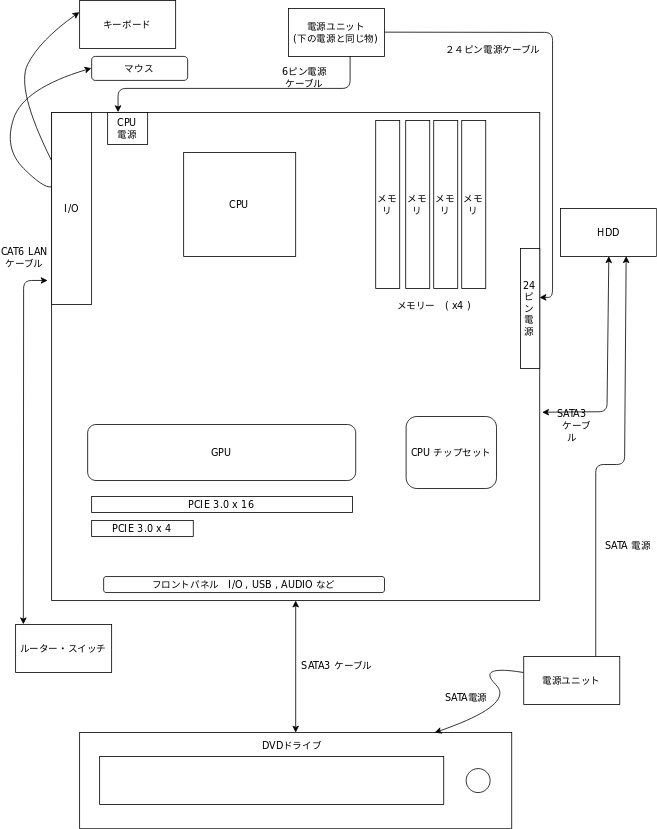
\includegraphics[width=0.704\textwidth]{pc.png}
			\caption{回路図}
		\end{figure}
	\section{実験方法}
		\subsection{電源の取り付け}
			\hspace{1cm} PCケースに電源を取り付ける。
		\subsection{CPUの取り付け}
			\hspace{1cm} マザーボードのCPUソケットにCPUを取り付けける。

\subsection{CPUファンの取り付け}
\hspace{1cm} CPUファンを取り付け、ファンの電源コネクターをマザーボードに接続する。			

\subsection{システムメモリの取り付け}
\hspace{1cm}マザーボードのメモリスロットにメモリの向きを合わせて差し込む
	

\subsection{マザーボードの取り付け}
\hspace{1cm}IOパネルをケースにつけた後にマザーボードをケースに取り付ける。


\subsection{GPUの取り付け}
\hspace{1cm}ケースのGPUスロットの金属プレートを取り外し、マザーボードのPCIEポートにGPUを差し込みねじで止める。


\subsection{ハードディスク(SSD)、光学ドライブの取り付け}
\hspace{1cm}2.5インチSSDに3.5インチ変換プレートを取り付けた後SSDをケースの3.5インチベイに取り付ける。そしてDVDドライブをドライブベイに取り付ける。

\subsection{各種ケーブルの接続}
\subsubsection{SATA,電源}\hspace{1cm} SATA電源ケーブルをSSDとドライブに接続する。次にSATAケーブル(データ)でSSDとドライブをマザーボードと接続する。マザーボードの SATA ケーブルコネクタの位置を図2に図示する。

\begin{figure}[H]
	\centering
	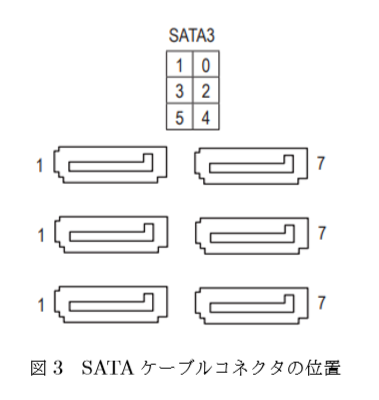
\includegraphics[width=5cm]{SATA.png}
	\caption{マザーボードSATAポート}
\end{figure}



\subsubsection{ATX電源ケーブル}
\hspace{1cm}マザーボードにATX電源(24ピン)とCPU電源(8ピン)ケーブルを接続する。コネクターの凸部とケーブルの凸部を同じ向きにして奥までしっかり差し込む。




\begin{figure}[H]
	\centering
	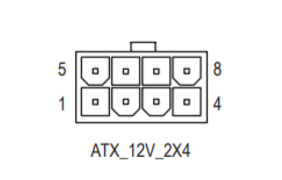
\includegraphics[width=5cm]{6PIN.png}
	\caption{ATX 12V 8ピン CPU電源}
\end{figure}

\begin{figure}[H]
	\centering
	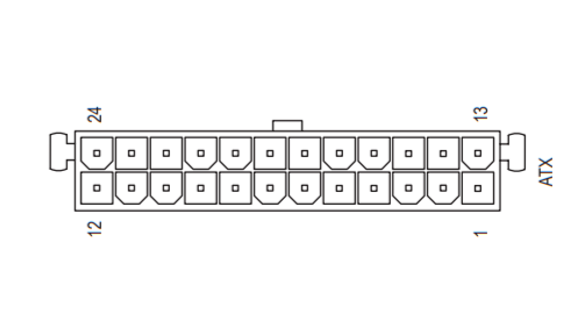
\includegraphics[width=5cm]{24PIN.png}
	\caption{ATX 24ピン 電源}
\end{figure}

\subsubsection{フロントパネルのUSBコネクタ}
\hspace{1cm}PCケースのフロントパネルのUSB2.0と3.0ケーブルをマザーボードピンヘッダーに接続する。

\begin{figure}[H]
	\centering
	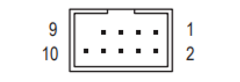
\includegraphics[width=5cm]{USB2}
	\caption{フロントパネル用USB2.0ヘッダー}
\end{figure}
\begin{figure}[H]
	\centering
	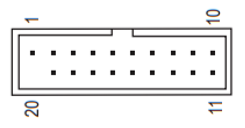
\includegraphics[width=5cm]{USB3}
	\caption{フロントパネル用USB3.0ヘッダー}
\end{figure}


\subsubsection{FANケーブル}
\hspace{1cm}マザーボードの4ピンファンヘッダーに、ケースファンの3ピンコネクターを接続する。

\begin{figure}[H]
	\centering
	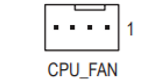
\includegraphics[width=5cm]{CPUFAN.png}
	\caption{CPU FAN ヘッダー}
	
\end{figure}

\begin{figure}[H]
	\centering
	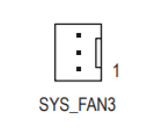
\includegraphics[width=5cm]{SYSFAN.png}
	\caption{ケースFAN ヘッダー}
	
\end{figure}

\subsection{LED及びスイッチケーブルの配線}
\hspace{1cm}マザーボードのピンヘッダにPOWER LED, HDD LED, POWERスイッチ、 リセットスイッチを接続する。

\begin{figure}[H]
	\centering
	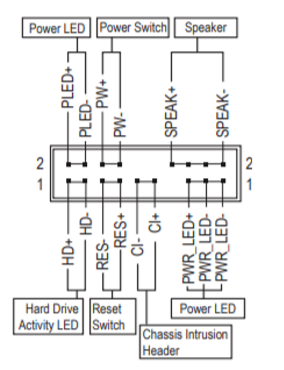
\includegraphics[width=5cm]{FRONT.png}
	\caption{LED/BUTTONヘッダー}
	
\end{figure}


\subsection{モニター、キーボード、マウスの取り付け}
\hspace{1cm}キーボードはPS2ポートに接続し、マウスはUSBポートに接続する。GPUのディスプレイコネクターにモニターケーブルを接続し、モニターには電源ケーブルを接続してからモニターの電源をつける。次に電源ユニットに電源ケーブルを接続してコンセントにつなぐ。ここまで終わったら指導員を読んで確認を依頼する。


\subsection{ 電源投入と BIOS の設定}
\hspace{1cm}			
 電源を ON にしその直後に「DEL」キーを連打すると BIOS 設定画面が表示される。 ここまでうまくいったらCPU電圧などの値を記録して、ボートデバイスからWidnowsのインストーラーをブートする。

\subsection{Windows 10 のインストール}
\hspace{1cm}Windows 10をSSDにインストールし、Windowsの初期設定を行う。

\subsection{解像度の調整}
\hspace{1cm}解像度は自動的に認識されていたため設定は行わなかった。

\subsection{ドライバーのインストール}
\hspace{1cm} スキップ

\subsection{ネットワークテスト}
\hspace{1cm}
\subsubsection{インターネットアクセステスト}
	インターネットにアクセスできているかを確認するため "www.c.dendai.ac.jp"などのウェブサイトをアクセスしてみる。 
\subsubsection{ipconfig}
	ipconfig /allでネットワークデバイスの情報を確認する。そしてその内容をUSBに保存する。

\subsection{分解}
\hspace{1cm}PCを分解して、パーツをもとの場所に戻す。

	
\pagebreak

\section{実験結果}
\subsection{ネットワークデバイス情報}
 \noindent\makebox[\linewidth]{\rule{\paperwidth}{0.4pt}}
 
\begin{alltt}
Windows IP 構成

ホスト名. . . . . . . . . . . . . . .: DESKTOP-T9QPT0L
プライマリ DNS サフィックス . . . . .: 
ノード タイプ . . . . . . . . . . . .: ハイブリッド
IP ルーティング有効 . . . . . . . . .: いいえ
WINS プロキシ有効 . . . . . . . . . .: いいえ
DNS サフィックス検索一覧. . . . . . .: localdomain

イーサネット アダプター イーサネット:

接続固有の DNS サフィックス . . . . .: localdomain
説明. . . . . . . . . . . . . . . . .: Killer E2500 Gigabit Ethernet Controller
物理アドレス. . . . . . . . . . . . .: 1C-1B-0D-A6-01-AC
DHCP 有効 . . . . . . . . . . . . . .: はい
自動構成有効. . . . . . . . . . . . .: はい
リンクローカル IPv6 アドレス. . . . .: fe80::a916:53fe:c945:8c8%3(優先) 
IPv4 アドレス . . . . . . . . . . . .: 133.20.42.19(優先) 
サブネット マスク . . . . . . . . . .: 255.255.255.128
リース取得. . . . . . . . . . . . . .: 2019年4月22日 19:26:44
リースの有効期限. . . . . . . . . . .: 2019年4月22日 22:29:57
デフォルト ゲートウェイ . . . . . . .: 133.20.42.126
DHCP サーバー . . . . . . . . . . . .: 133.20.42.120
DHCPv6 IAID . . . . . . . . . . . . .: 52173581
DHCPv6 クライアント DUID. . . . . . .: 00-01-00-01-24-4F-4F-36-1C-1B-0D-A6-01-AC
DNS サーバー. . . . . . . . . . . . .: 133.20.97.40
133.20.97.70
NetBIOS over TCP/IP . . . . . . . . .: 有効

Tunnel adapter Teredo Tunneling Pseudo-Interface:

接続固有の DNS サフィックス . . . . .: 
説明. . . . . . . . . . . . . . . . .: Teredo Tunneling Pseudo-Interface
物理アドレス. . . . . . . . . . . . .: 00-00-00-00-00-00-00-E0
DHCP 有効 . . . . . . . . . . . . . .: いいえ
自動構成有効. . . . . . . . . . . . .: はい
IPv6 アドレス . . . . . . . . . . . .: 2001:0:348b:fb58:30a6:2357:7aeb:d5ec(優先) 
リンクローカル IPv6 アドレス. . . . .: fe80::30a6:2357:7aeb:d5ec%7(優先) 
デフォルト ゲートウェイ . . . . . . .: ::
DHCPv6 IAID . . . . . . . . . . . . .: 117440512
DHCPv6 クライアント DUID. . . . . . .: 00-01-00-01-24-4F-4F-36-1C-1B-0D-A6-01-AC
NetBIOS over TCP/IP . . . . . . . . .: 無効
\end{alltt}
\noindent\makebox[\linewidth]{\rule{\paperwidth}{0.4pt}}


\subsection{BIOSのCPUとメモリー情報}
\begingroup
\setlength{\tabcolsep}{10pt} % Default value: 6pt
\renewcommand{\arraystretch}{1.5} % Default value: 1
\begin{table}[H]
	\caption{ハードウェア情報}
	\centering
	\begin{tabular}{|l|l|}
		\hline
		Processor Type & Intel Celeron \\ \hline
		CPUID & 906E9H \\ \hline
		CPU Speed & 2900.96Mhz \\ \hline
		Installed Memory & 8192MB \\ \hline
		Model Name & H270 Gaming 3 \\ \hline
		BIOS Version & F2 \\ \hline
		BIOS ID & 8A1BAG03 \\ \hline
		Mac Address & 1C1B0DA601AC \\ \hline
	\end{tabular}
\end{table}
\endgroup


\subsection{ブートデバイス情報}
\begingroup
\setlength{\tabcolsep}{10pt} % Default value: 6pt
\renewcommand{\arraystretch}{1.5} % Default value: 1
\begin{table}[H]
	\caption{ブートデバイス}
	\centering
	\begin{tabular}{|l|l|}
		\hline
		UEFI & Optiarc DVD RW AD-7260S \\ \hline
		P2   & TS128GSSD230S           \\ \hline
		P3   & Optiarc DVD RW AD-7260S \\ \hline
	\end{tabular}
\end{table}
\endgroup


\subsection{CPU電圧、CPU温度、ファン回転速度など}
\begingroup
\setlength{\tabcolsep}{10pt} % Default value: 6pt
\renewcommand{\arraystretch}{1.5} % Default value: 1
\begin{table}[H]
	\caption{PCの健康状態}
	\centering
	\begin{tabular}{|l|l|}
		\hline
		CPU Vコア & 0.936V \\ \hline
		3.3V   & 3.363V           \\ \hline
		5V   & 5.100V \\ \hline
		12V   & 12.168V \\ \hline
		CPU温度   & 36.0\textdegree{}C \\ \hline
		FAN SPEED  & 1290RPM \\ \hline
	\end{tabular}
\end{table}
\endgroup
\pagebreak

\section{検討事項}
\subsection{ストアドプログラム方式}
\hspace{1cm} プログラム命令をRAMなどの主記憶装置に保存し、その命令を実行するコンピュータアーキテクチャ方式である。(ノイマン型アーキテクチャ、ハーバードアーキテクチャなど)
\subsection{OSの目的と機能}
\subsubsection{目的}
$\bullet$ システム上にあるチップ、記憶装置などを制御する役割を果たしている。 システム上のパーツをすべて制御し、それらのパーツへのインターフェースをAPIをして提供しており、これ使うことによってソフトの開発者が数多くCPUアーキテクチャや記憶装置別にプログラムを書かなくてすむ。また、TCP・IPの実装やシステムクロックの制御などもすべてOSがやってくれていて、もしプログラマが時間を取得したい場合はAPIコールでシステムに要求すれば簡単に取得できる。\\
$\bullet$プログラムが任意にメモリをアクセスできないようにしたり(セグメンテーション)、使わなくなったメモリを開放したりすることによってセキュリティーやパフォーマンスが向上される。

\subsubsection{機能}
$\bullet$ ファイルエクスプローラーなどを使うことによってCUIに触れなくてもファイルを簡単に操作できる。\\
$\bullet$ GUIを使うことによってパソコンの知識(開発)が詳しくない人でもプログラムを容易にインストールしたり、システムの設定を変えたりすることができる。\\
$\bullet$ CPUアーキテクチャなどが異なるパソコンどうしで同じアプリを使うことができる。\\
$\bullet$ 記憶装置やハードウェアの健康状態をモニタリングし(S.M.A.R.Tなど)、異常があるときに注意してくれる。

\section{吟味 (考察)}
$\bullet$ 今までは主にLGA2011やAMDのシステムしか組んだことなかったので本実験では、LGA1151ソケットにCPUクーラーを取り付ける方法を理解しました。

\end{document}




% \begin{verbatim}
%このテキストは、別のフォントを持つことになります
%This is a verbatim environment with mono-space font
%\end{verbatim} 
